\section{Diseño-experimental}

	\subsection{Grupos de estudio}

	\begin{frame}
	    \frametitle{Grupos de estudio}
	    \vspace*{2mm}
	    \textbf{\large Agua}\\[5mm]  
	    
	    Las muestras de agua se seleccionaron guiándose en la clasificación propuesta por la \acrfull{wqa}. Se proponen 3 grupos para evaluar los casos límite y promedio de la salinidad del agua de mar.
	      
	    \begin{longtblr}[
			caption = {Grupo de control del agua de mar},
			label = {table:grupo-control-agua}
		]{
			colspec = {X[c] X[2, c]},
			hlines,
			vlines,
			width = 0.5\linewidth,
			rowhead = 1,
			row{odd} = {bg=tablerowblue},
			row{1} = {
				bg = tabletitleblue,
				fg=white,
				font = \bfseries,
				halign=c
			},
			rows={m}
		}
			Muestra & Salinidad (\unit{\mg\per\litre})\\
			1 & \num{30000}\\
			2 & \num{35000}\\
			3 & \num{40000}
		\end{longtblr}
	\end{frame}
	
	\begin{frame}
	    \frametitle{Lugar físico de experimentación}
	    \vspace*{2mm}
	    
	    Unidad Profesional Interdisciplinaria en Ingeniería y Tecnologías Avanzadas ubicada en la Ciudad de México.
			
			\begin{longtblr}[
				caption = {Grupo de control del agua de mar},
				label = {table:grupo-control-fisico}
			]{
				colspec = {X[c] *{3}{c}},
				hlines,
				vlines,
				width = 0.8\linewidth,
				rowhead = 1,
				row{odd} = {bg=tablerowblue},
				row{1} = {
					bg = tabletitleblue,
					fg=white,
					font = \bfseries,
					halign=c
				},
				rows={m}
			}
				Zona & Longitud & Latitud & Altitud\\
				Ciudad de México, México
					& \ang{-99;07;32}
					& \ang{19;30;38}
					& \qty{2241}{\m}
			\end{longtblr}
	    
	\end{frame}
	
	
		
	\subsection{Propuesta de diseño}
	\begin{frame}
	    \frametitle{Diseño del desalinizador}
	    \vspace*{2mm}
	    
	    \begin{figure}
		    	\centering
		    	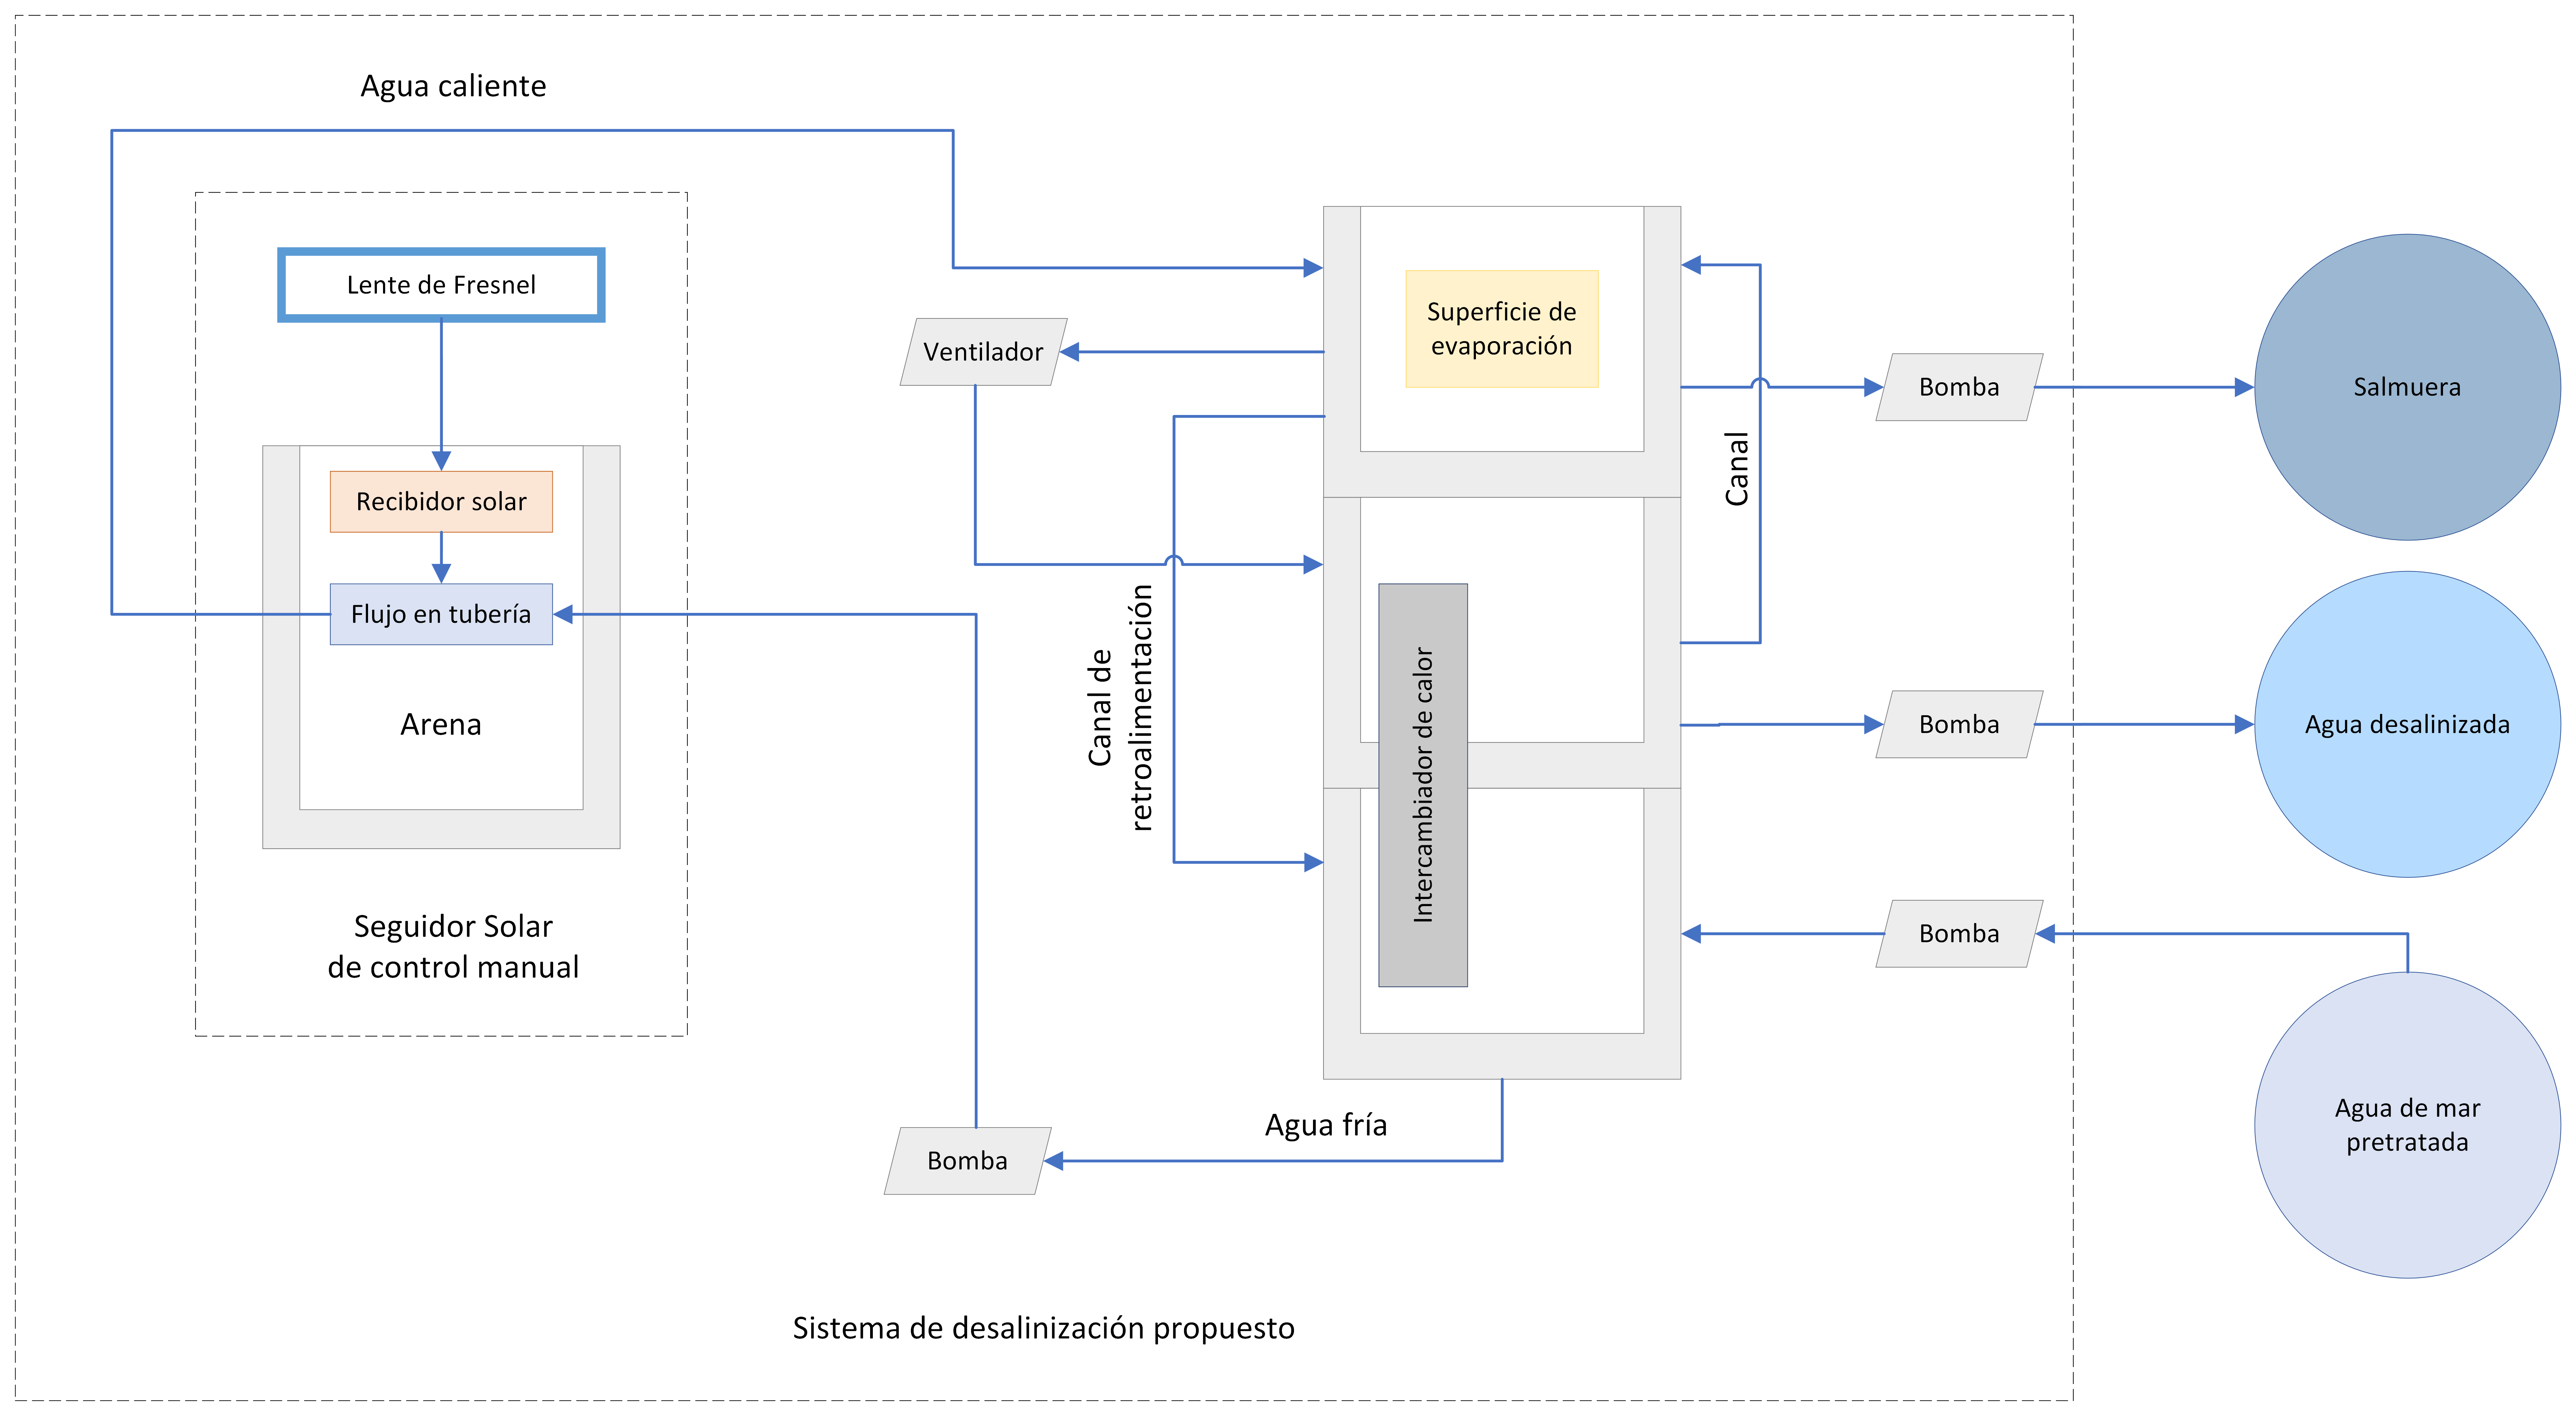
\includegraphics[
			    	width=\linewidth,
			    	height = 60mm,
			    	keepaspectratio
			]{Resultados/Sistema/VistaGeneral.png}
			\caption{Diagrama de funcionamiento del desalinizador}
	    \end{figure}		
	\end{frame}
	
	\begin{frame}
		\frametitle{Módulo de reaprovechamiento térmico y bombeo}
		\vspace*{2mm}
		
		\begin{figure}
		    	\centering
		    	\only<1>{
		    	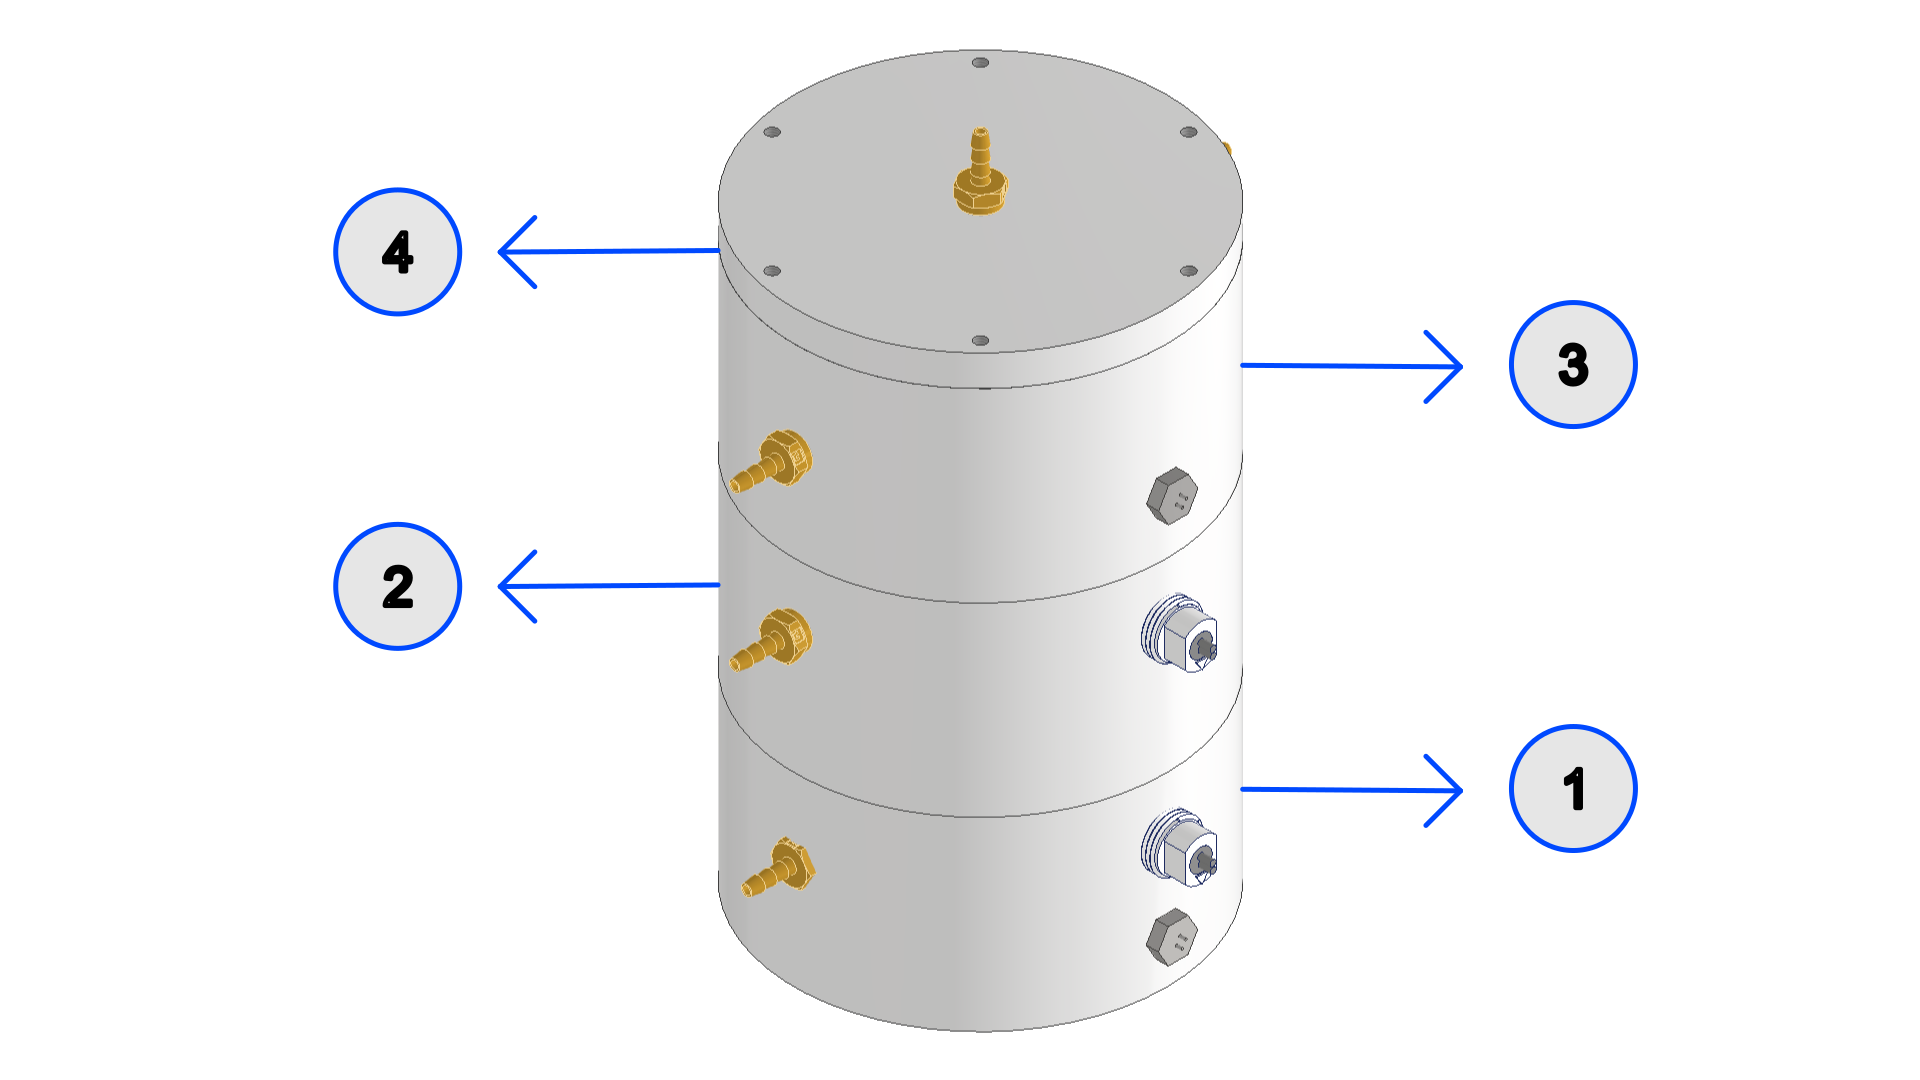
\includegraphics[
			    	width=\linewidth,
			    	height = 60mm,
			    	keepaspectratio
			]{Resultados/Sistema/WaterModule.png}
			\caption{Submódulos}
			}
			\only<2>{
		    	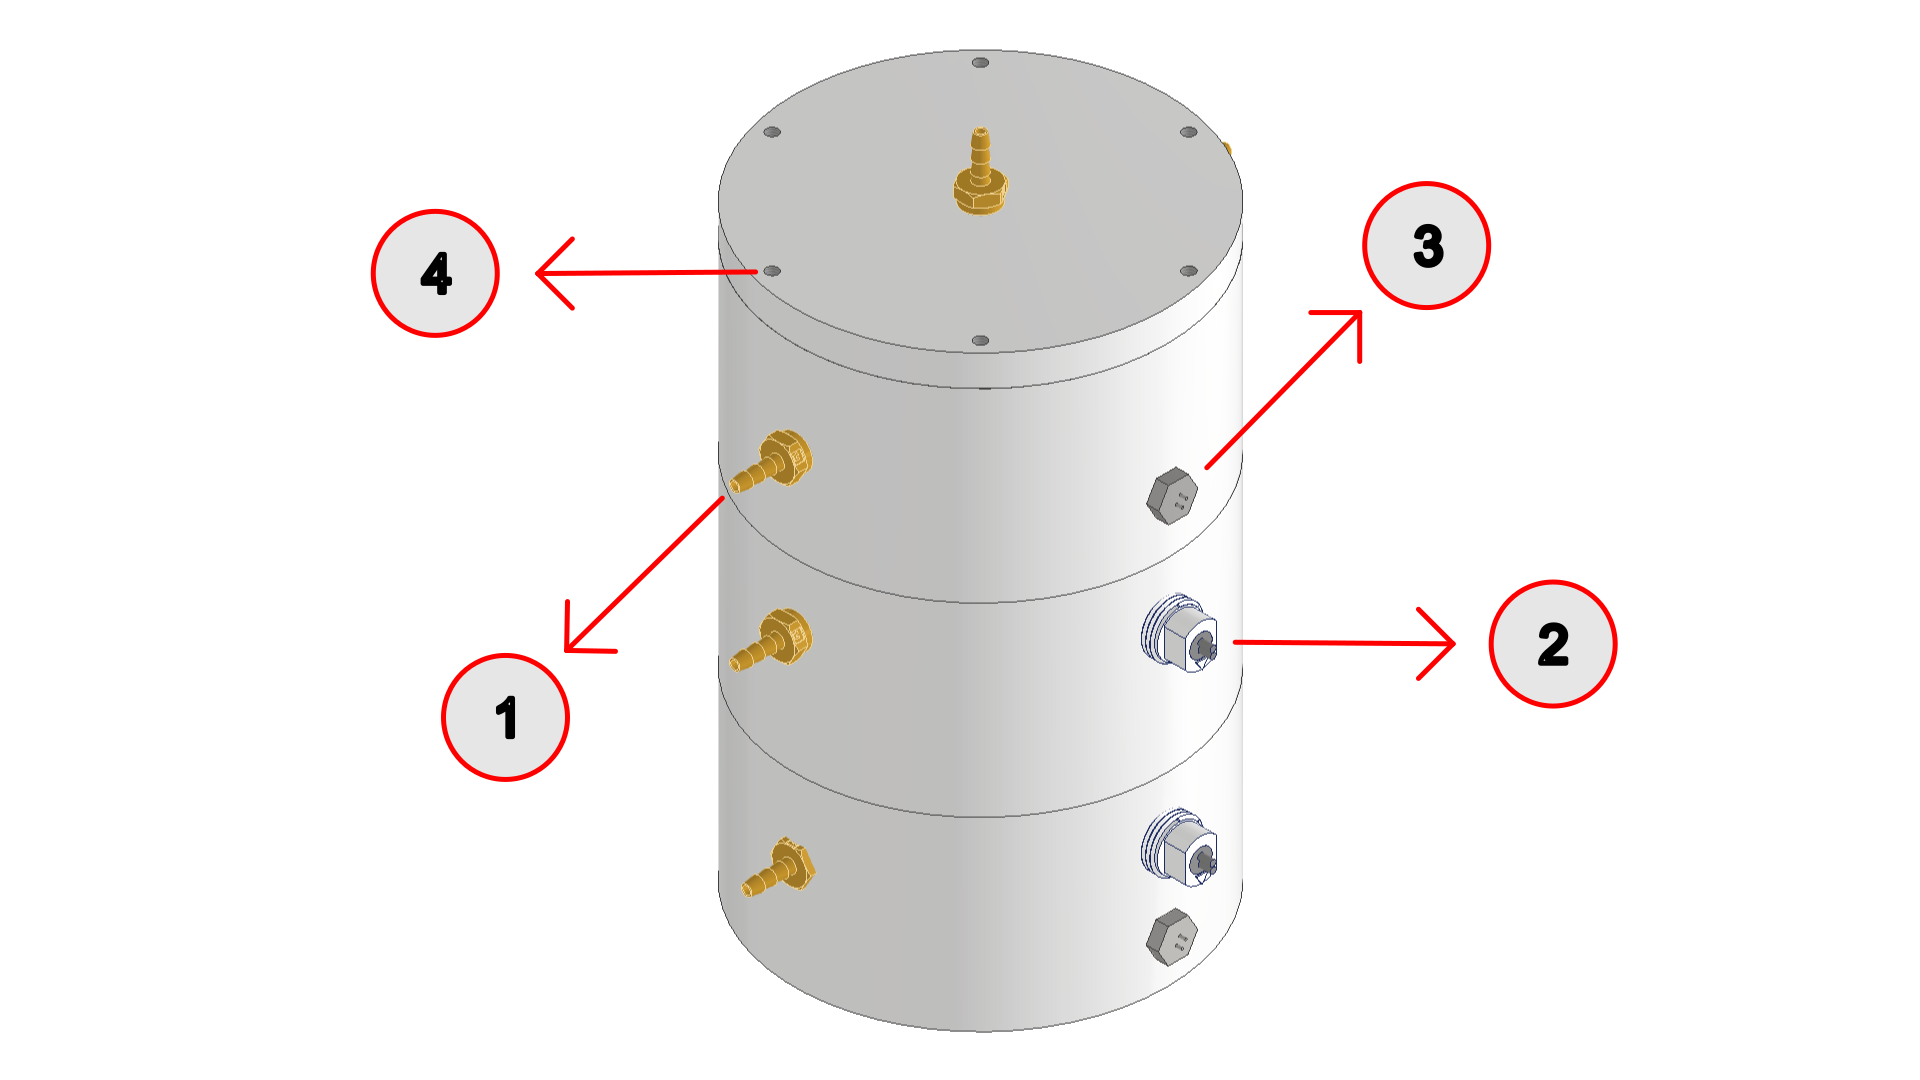
\includegraphics[
			    	width=\linewidth,
			    	height = 60mm,
			    	keepaspectratio
			]{Resultados/Sistema/WaterModuleComponents.png}
			\caption{Componentes}
			}
	    \end{figure}
	\end{frame}
	
	\begin{frame}
		\frametitle{Módulo de concentración solar}
		\vspace*{2mm}
		
		\begin{figure}
		    	\centering
		    	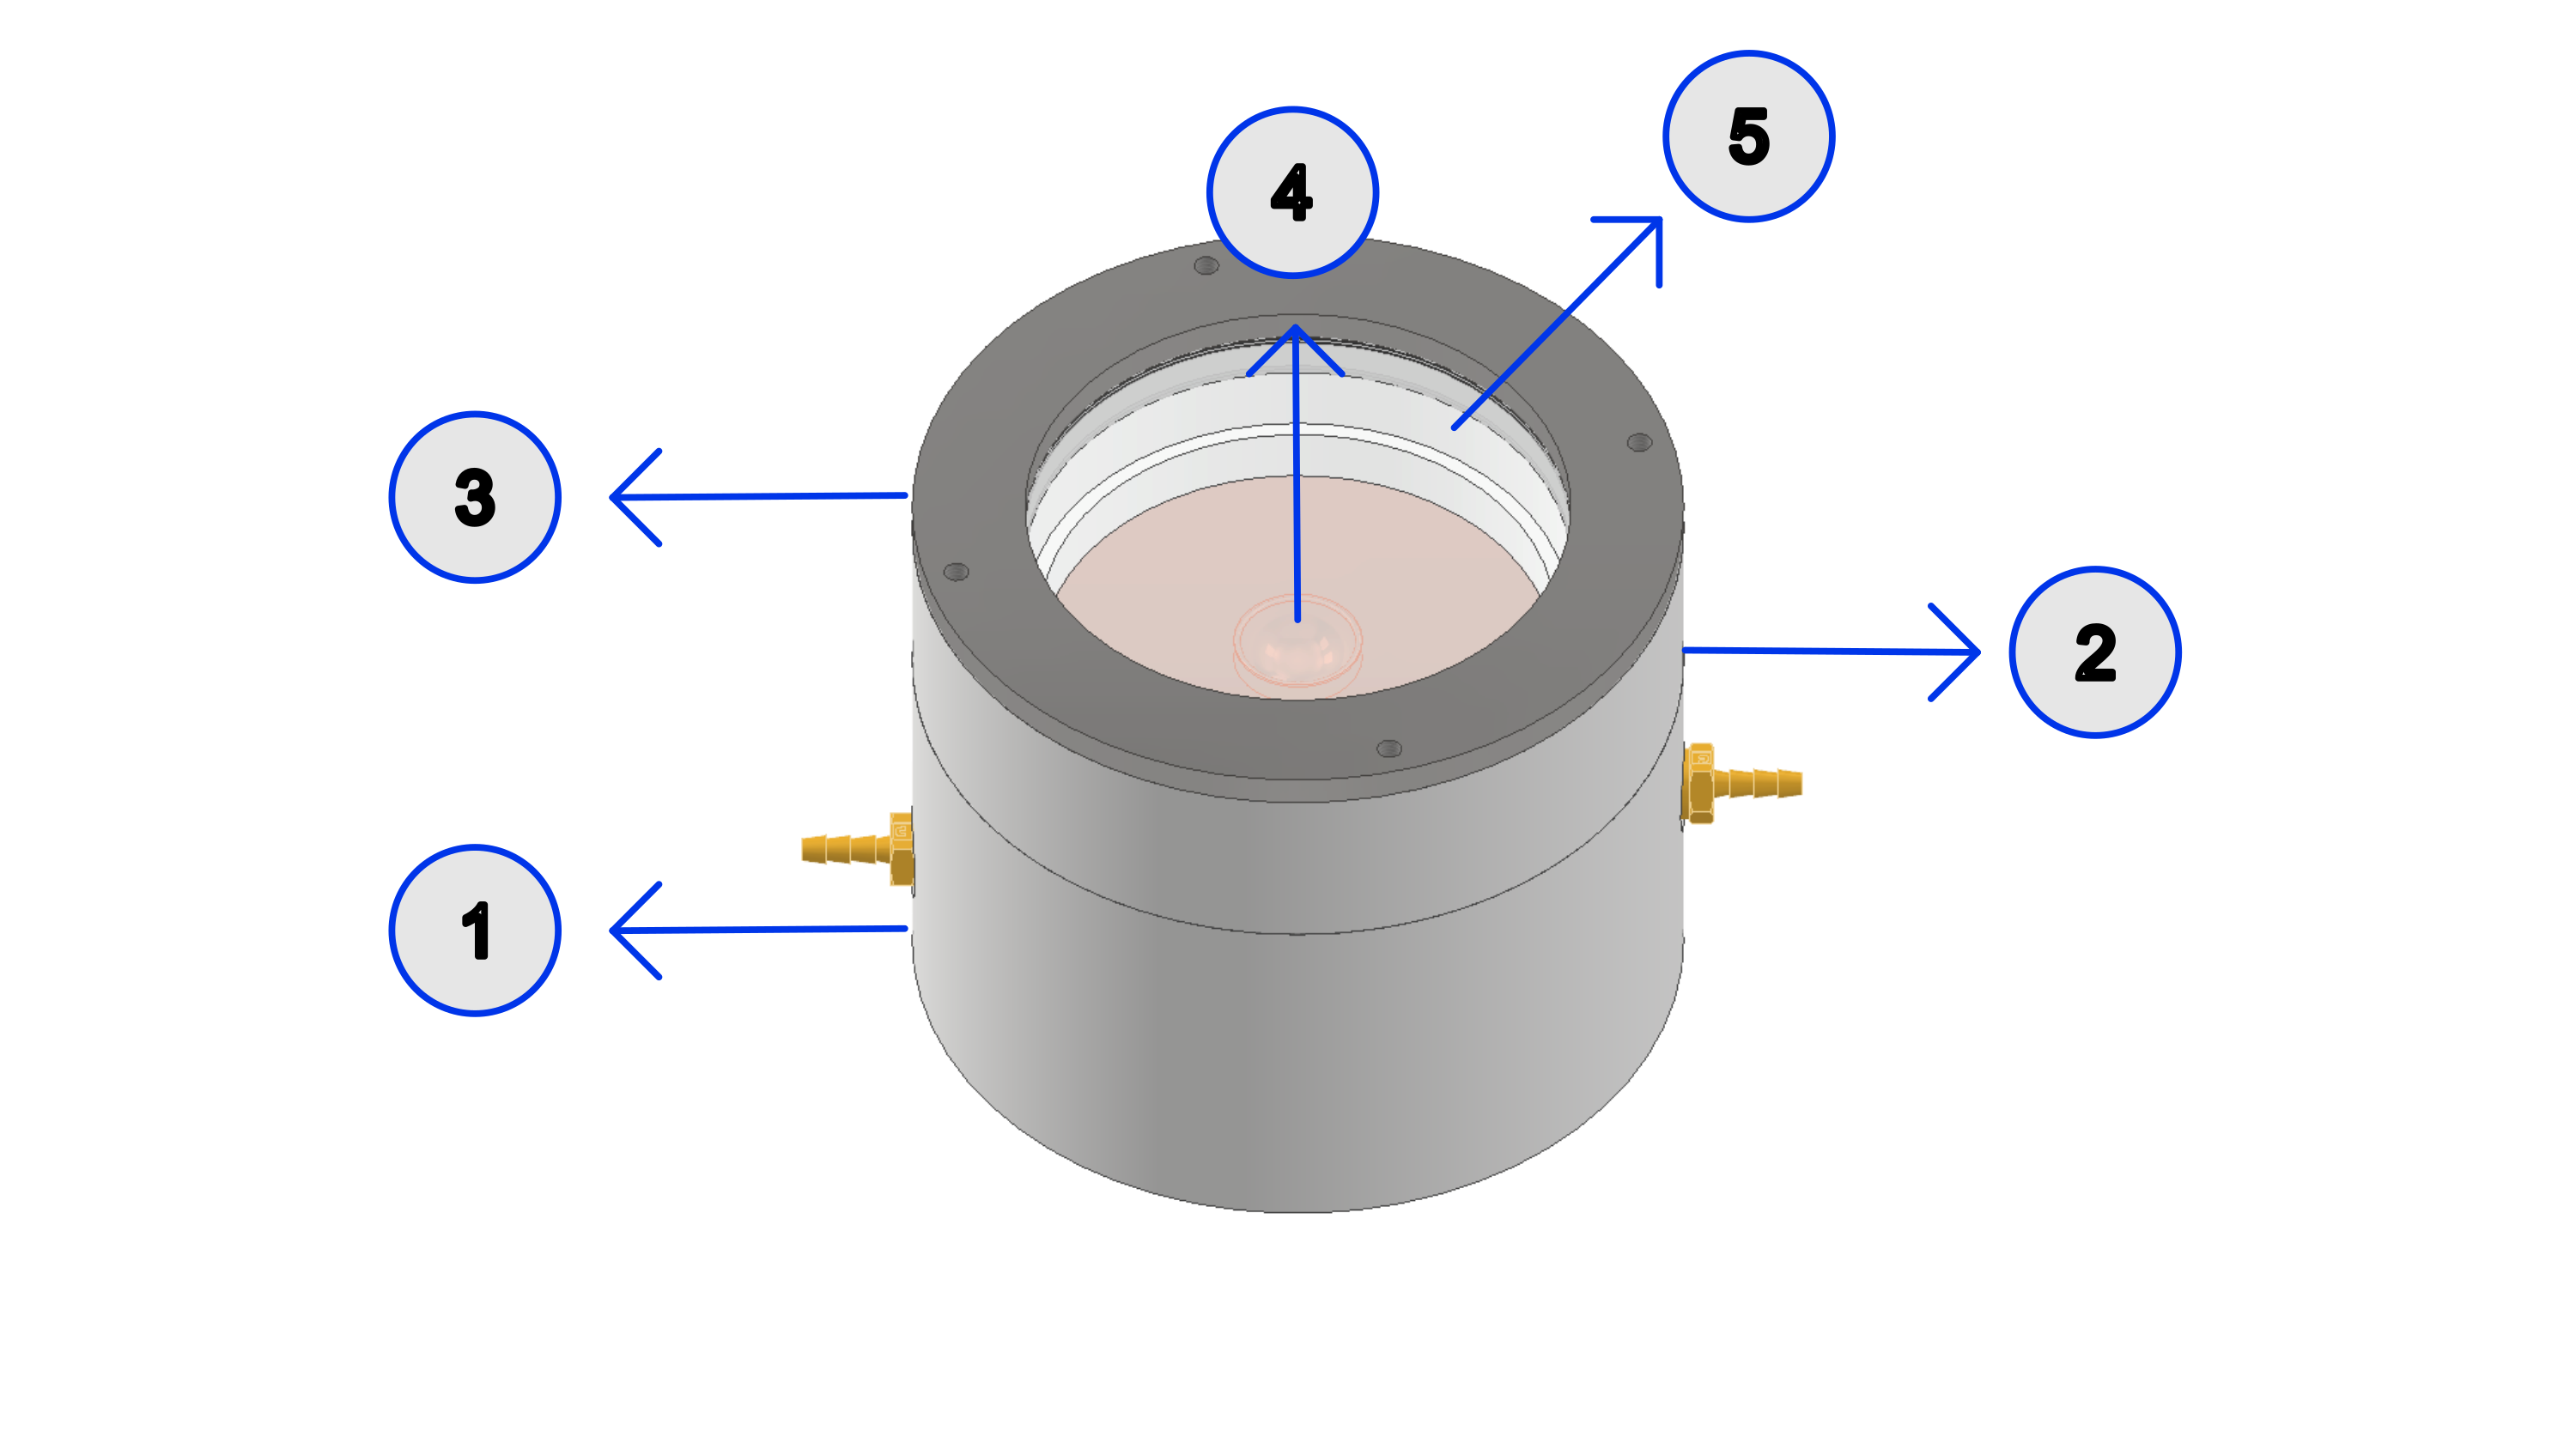
\includegraphics[
			    	width=\linewidth,
			    	height = 60mm,
			    	keepaspectratio
			]{Resultados/Sistema/SolarModule.png}
			\caption{Submódulos}
	    \end{figure}
	\end{frame}
	
	\begin{frame}
		\frametitle{Simulaciones}
		\vspace*{2mm}
		\begin{columns}
	    		\begin{column}{0.5\linewidth}
	    			\begin{figure}
	    				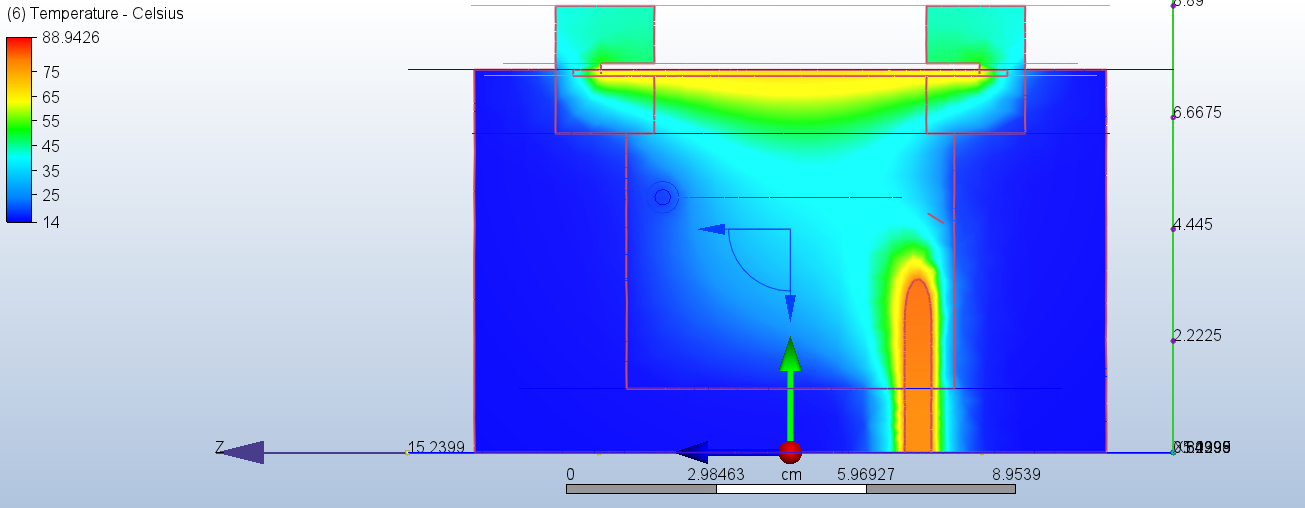
\includegraphics[
		    				width=\linewidth
	    				]{Resultados/Simulaciones/50WCopper15C9mlpm.png}
	    				\caption{Corte en la entrada y salida del agua de mar usando una tubería de cobre}
	    			\end{figure}
		    \end{column}
		    \begin{column}{0.5\linewidth}
		    		\begin{figure}
	    				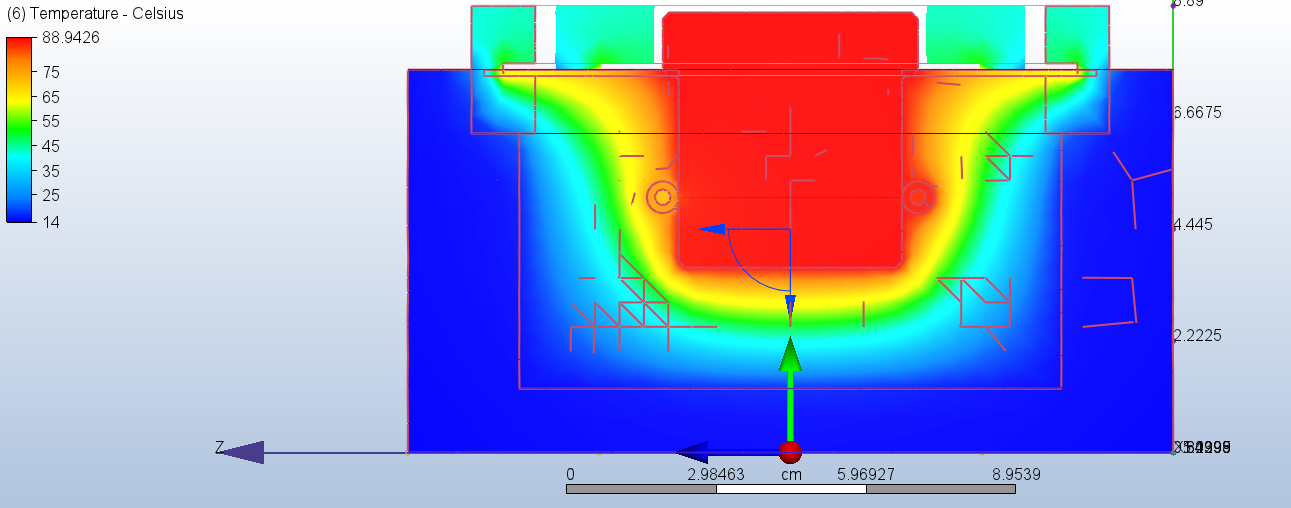
\includegraphics[
		    				width=\linewidth
	    				]{Resultados/Simulaciones/50WCopper15C9mlpm-middle.png}
	    				\caption{Corte en el centro del recibidor solar y su transferencia de calor hacia el cobre}
	    			\end{figure}
		    \end{column}
	    \end{columns}
	\end{frame}
	
	\begin{frame}
		\frametitle{Simulaciones}
		\vspace*{2mm}
		\begin{figure}
    			\includegraphics[
    				width=\linewidth,
    				height = 6cm,
    				keepaspectratio
    			]{Resultados/Simulaciones/FuzzyUniverse.png}
    			\caption{Simulaciones posteriores para determinar el universo de discurso del control difuso}
  		\end{figure}
	\end{frame}